%=========================================================================
%Jakub Bartecek (xbarte09)
%Date: 2013 - 2014
%Encoding: UTF-8
%set syntax=tex
%\listoffigures

\chapter{Úvod}
    Tato diplomová práce se zabývá vylepšením serveru Jenkins CI, který je v~praxi využíván pro potřeby průběžného testování softwaru
    a~jeho kontinuální integraci. Vylepšení se týká především webového serveru a~\emph{servlet} kontejneru, který je v~Jenkins CI integrován. 
    V~současném stavu tyto funkce vykonává kombinace serverů Winstone a~Jetty. 
    
    Server Winstone je již neudržovaný a~zastaralý nástroj a~z~tohoto důvodu
    byl z~velké části nahrazen serverem Jetty, který potřebnou funkcionalitu poskytuje. Server Jetty je poměrně komplexní projekt a~nabízí
    mnoho funkcionality, ale na druhou stranu jeho rozsah nedovoluje poskytovat maximální rychlost.
    
    V~současné době vznikl nový webový server Undertow, který si klade za cíl být co nejjednodušší a~nejrychlejší a~mohl by být přínosný
    a~vhodný pro Jenkins CI. Jelikož tento server je nový a~je sponzorován firmou Red Hat, tak lze předpokládat, že jeho vývoj
    bude nadále pokračovat a~nebude zastarávat.

    Cílem této práce je nahradit server Jetty a~případně i~server Winstone pomocí serveru Undertow 
    a~integrovat jej se serverem Jenkins CI. Při integraci je kladen důraz na snahu
    zachovat zpětnou kompatibilitu s~původním řešením. 

    V~rámci této diplomové práce jsou nejprve rozebírány potřebné informace týkající se jednotlivých nástrojů a~plánované integrace.
    Následně je detailně analyzována architektura Jenkins CI a~způsob jeho integrace se servery Winstone a~Jetty. V~navazující části
    je diskutována varianta nahrazení pouze serveru Jetty a~varianta nahrazení serveru Jetty i~Winstone pomocí serveru Undertow. 
    Z~provedené analýzy byla zvolena jedna varianta, která byla vybrána pro následnou integraci. 

    %TODO popis implementace a performance testování

    



%%%%%%%%%%%%%%%%%%%%%%%%%%%%%%%%%%%%%%%%%%%%%%%%%%%%%%%%%%%%%%%%%%%%%%%%%%%%%%%%%%%%%%%%%%%%%%%
%%%%%%%%%%%%%%%%%%%%%%%%%%%%%%%%%%%%%%%%%%%%%%%%%%%%%%%%%%%%%%%%%%%%%%%%%%%%%%%%%%%%%%%%%%%%%%%
\chapter{Jenkins CI a~související nástroje}
    Tato kapitola se zaměřuje na teoretické základy práce, které je nutné nebo vhodné znát pro pochopení zpracovávané problematiky.
    Je zde detailněji popsán systém Jenkins CI (kapitola~\ref{jenkins}) ke kterému se tato práce přímo váže. S~ním je spojeno seznámení
    se servery Winstone (kapitola \ref{winstone}) a~Jetty (kapitola \ref{jetty}), jejichž kombinace je současně v~Jenkins CI integrována.
    Po popisu těchto serverů je rozebírán průběh jejich využití v~servlet kontejneru Jenkins CI a~průběh jeho vývoje (kapitola \ref{vyvojWinstone}). 
    V~kapitole \ref{servletWebserver} jsou vysvětleny často zde používané pojmy \emph{servlet kontejner} a~webový server.

    Větší důraz je dále věnován serveru Undertow (kapitola \ref{undertow}), který byl vybrán jako nový webový server pro Jenkins CI. V~tomto případě je provedena hlubší studie
    tohoto nástroje, aby na jejím základě bylo možné pochopit a~provést samotnou integraci s~Jenkins CI, která je jádrem této práce. 
    %Pro poskytnutí ucelených informací
    %je menší prostor také vymezen pro nástroj Maven (kapitola \ref{maven}), který se používá k řízení překladu serveru Jenkins CI, a je v této práci několikrát zmiňován. 

    Uvedené informace mají spíše informativní charakter, aby poskytly ucelený úvod do zkoumané problematiky. Jsou zaměřeny především na informace týkající se samotné
    integrace. Pro případné získání detailnějších informací jsou uvedeny patřičné zdroje, kde je lze nalézt.

    %%%%%%%%%%%%%%%%%%%%%%%%%%%%%%%%%%%%%%%%%%%%%%%%%%%%%%%%%%%%%%%%%%%%%%%%%%%%%%%%%%%%%%%%%%%%%%%
    \section {Jenkins CI} \label{jenkins}
        Jenkins CI je komunitní open source nástroj pro kontinuální integraci softwaru, který je vyvíjen pod svobodnou licencí
        MIT\footnote{Licence MIT: \texttt{http://opensource.org/licenses/MIT}} \cite{jenkinsGovernance}.
        Je velmi populární a~využíván malými i~velkými firmami jako je například firma Red Hat, kde tento program běží na stovkách serverů.
        Původní název tohoto projektu je Hudson\footnote{Webové stránky projektu Hudson: \texttt{http://hudson-ci.org/}}. 
        Když se jeho vývoje ujala firma Oracle, tak se projekt
        rozštěpil a~vznikla jeho komunitní verze, kterou je projekt Jenkins CI. Přesto se v~některých částech tohoto projektu 
        stále objevuje název Hudson, ale jedná se pouze pozůstatek z~původního projektu.

        Zkratka CI je z~anglického spojení \emph{continuous integration}, což lze do češtiny přeložit jako kontinuální nebo průběžná 
        integrace. Krátké seznámení s~touto metodologií je v~následující kapitole.

        Informace v~této kapitole byly čerpány především  z~knihy \cite{jenkinsBook}, kde lze nalézt další informace o~serveru Jenkins CI,
        a~také z~webové stránky projektu \cite{jenkinsWeb}.

        \subsection{Kontinuální integrace a~využití Jenkins CI}
            V~minulosti byla integrace programu do výsledného produktu velmi náročným procesem a~často ztraceným časem.
            S~vydáním každé verze programu se musel postup probíhající před vydáním produktu opakovat a~pro vývojářský tým
            to prakticky znamenalo zdržení. Pokud se v~tomto procesu odhalil nějaký problém (což bylo běžné),
            tak jeho řešení bylo z~důvodu nedostatku času a~jeho pozdního objevení mnohem problematičtější
            než kdyby byl tento problém odhalen dříve.

            Kontinuální integrace je moderní přístup k~vývoji softwaru, který mění způsob přemýšlení nad celým procesem vývoje
            a~snaží se předcházet problémům popsaným výše a~především ušetřit čas. V~tomto přístupu je využíván nějaký
            kvalitní nástroj, který automatizovaně provádí specifikované kroky, které provázejí integraci softwaru a~jeho vydání.

            Jedním z~nástrojů poskytujích podporu pro kontinuální integraci při vývoji softwaru je 
            server Jenkins CI. 
            
            \medskip \noindent Základními možnostmi, které umožňuje Jenkins CI nakonfigurovat, jsou:
            
            \begin{itemize}
                \item Spouštění integračních a~jednotkových testů v~přesně definovaném čase (např. v~noci, kdy jsou servery méně vytížené)
                \item Spuštění integračních a~jednotkových testů při změně ve verzovacím systému. Jenkins CI dokáže zaznamenat změnu v~repozitáři,
                    stáhnout si změny a~spustit testování
                \item Shromažďování a~vyhodnocování metrik vývoje softwaru
                \item Spuštění akceptačních testů
                \item Informování e-mailem o~testech, které skončily chybou
                \item Automatické nahrání nové verze produktu na server
            \end{itemize} 

            Uživatelé mohou kdykoliv přidat využití libovolné funkcionality systému a~neopakovat stále stejné kroky. 
            

        \subsection{Způsoby použití aplikace}
            Celý program je napsán v~jazyce Java a~je tedy plně přenositelný mezi platformami. Architektura je navržena tak, aby byla 
            lehce rozšiřitelná pomocí tzv. \emph{pluginů}, kterých je pro něj vytvořené velké množství. 
            
            Jenkins CI je určen pro běh na serveru a~je dostupný přes webové rozhraní (ale může být samozřejmě spuštěn
            na libovolném osobním počítači). Komunikuje pomocí protokolu \emph{HTTP}, 
            který je založen na modelu \emph{požadavek-odpověď} (angl. \emph{request-response}). Jelikož tento způsob komunikace
            je velmi běžný, tak není v~programu přímo implementován, ale využívá k~němu externí nástroje. 
            Dalším nástrojem, který pro svou činnost Jenkins potřebuje, je servlet kontejner ve kterém samotná 
            aplikace poběží.
            Tento pojem je blíže objasněn v~kapitole \ref{servletWebserver}.

            \medskip \noindent
            Existují dvě možnosti jak spustit server Jenkins CI:

            \begin{enumerate}
                \item{Může běžet na libovolném \emph{Java EE} aplikačním serveru \cite{jenkinsServers} jako jsou například servery 
                JBoss\footnote{Více informací o~serveru viz \texttt{http://www.jboss.org/jbossas/}} 
                anebo Glasfish\footnote{Více informací o~serveru viz \texttt{http://www.oracle.com/technetwork/middleware/glassfish/}}}.
                Jenkins CI se standardně nasadí na server (dle zvyklostí konkrétního serveru)
                a~poté je s~ním možné pracovat. V~tomto případě veškerou nízkoúrovňovou komunikaci pomocí síťových protokolů 
                i~práci servlet kontejneru zajišťuje aplikační server.
                
                \item{Pokud nechceme nebo nemůžeme spouštět Jenkins CI na aplikačním serveru, tak jej lze spustit přímo
                    z~vytvořené \texttt{.war} archivu (překladem se zabývá kapitola \ref{jenkinsUsage}). V~tomto případě
                    se o~práci servlet kontejneru i~webového serveru komunikujícího jedním ze standardních síťových protokolů stará 
                    kombinace nástrojů Winstone a~Jetty, které jsou přímo integrovány do serveru Jenkins CI. 
                    
                    Nahrazení těchto dvou nástrojů (nebo pouze serveru Jetty) a~zajištění vykonávání této činnosti je hlavním cílem této práce.
                    Záměrem je tedy nahradit server Jetty a~případně i~server Winstone pomocí zvoleného nového serveru Undertow.
                    Studie těchto nástrojů a~jejich rozbor je předmětem následujícíh kapitol.}
            \end{enumerate}

            Pro tuto práci je důležitý druhý způsob používání Jenkins CI a~proto další informace se budou přímo vázat k~němu.

         \subsection{Architektura serveru}   \label{secJenkinsArchitektura}
            Architektura systému Jenkins CI je poměrně komplikovaná a~pro tuto práci není nutné ji detailně celou znát.
            Bude popsána na vysoké úrovni abstrakce a~zaměří se pouze na komponenty, které se přímo týkají této práce
            a~budou dále v~textu odkazovány nebo blíže rozebírány. Přehled architektury je na obrázku~\ref{imgJenkinsArchitecture}.
       
            \begin{figure}[ht]
                \begin{center}
                    \scalebox{0.65}{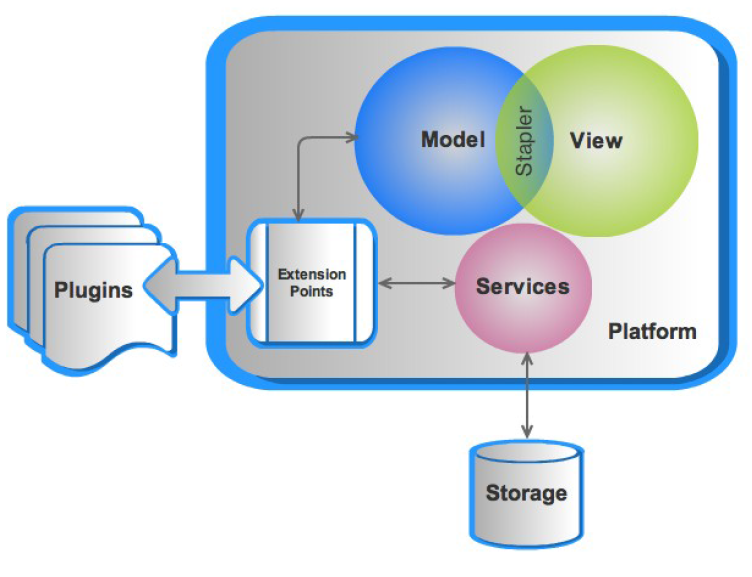
\includegraphics{img/jenkinsArchitecture.png}}
                    \caption{Přehled architektury serveru Jenkins CI \cite{architectureOverview}}
                    \label{imgJenkinsArchitecture}
                \end{center}
            \end{figure}     

            Základem architektury je část \emph{Model}, což jsou objekty, které obsahují stav
            a~data aplikace. Každý model je přímo navázán na konkrétní URL adresu s~tím, že kořenový
            model (dostupný pod URL \uv{/}) je pevně daná instance s~názvem \texttt{Hudson}.
            Data z~objektů modelu jsou následně zobrazovány ve webovém rozhraní aplikace.
            Pro toto zobrazování je využita techonologie Jelly.

            Velmi podstatnou součástí aplikace je prvek \emph{Stapler}. Tento objekt
            provádí konkrétní propojování požadavků dle zadané URL s~patřičnými objekty
            z~modelu a~spouštění vykonávání jejich metod. Stapler je
            jediným servletem, který je v~aplikaci Jenkins CI zaveden do
            servlet kontejneru při spuštění aplikace (pojmy servlet a~servlet kontejner 
            jsou vysvětleny v~kapitole \ref{servletKontejner}).
            Povědomí o~jeho
            činnosti je potřebné, protože s~ním bude v~této práci dále pracováno.
            Průběh vybírání patřičných metod pomocí této komponenty je přesně
            definován a~lze jej najít v~uživatelské příručce\footnote{
                Způsob zpracovávání požadavků komponentou Stapler:
                \texttt{http://stapler.kohsuke.org/reference.html}}, 
                ale není nutné jej zde rozebírat.

            Architektura serveru je přizpůsobena tak, aby byla snadno rozšiřitelná
            pomocí rozšiřujících modulů (angl. \emph{plugins}). Popis technologie Jelly
            i~tvorba rozšiřujících modulů je nad rámec této práce a~lze tyto informace
            najít v~odkazované literatuře.
        
            Informace v~této kapitole byly čerpány z~tohoto dokumentu \cite{architectureOverview}
            a~z~webových stránek projektu Stapler \cite{staplerWeb}.

        \subsection{Základy práce s~Jenkins CI} \label{jenkinsUsage}
            Pro přeložení a~spuštění aplikace je potřeba pracovat z~příkazové řádky nebo provést instalaci nějakým dávkovým souborem (skriptem).
            Aplikaci je možné stáhnout připravenou přímo ze stránek projektu \cite{jenkinsWeb}, ale pro tuto práci je potřeba 
            pracovat s~aplikací ze zdrojových souborů. Aktuální verze aplikace je dostupná na serveru 
            GitHub\footnote{Adresa aktuální verze Jekins CI: \texttt{www.github.com/jenkinsci}}.

            Po stažení zdrojových souborů je potřeba provést překlad aplikace. Pro tento automatizovaný 
            překlad se používá nástroj Maven\footnote{Více informací o~nástroji Maven lze získat na stránce 
            \texttt{http://maven.apache.org/}},který je krátce zmíněn v kapitole \ref{maven}. 
            
            Překlad aplikace bez spuštění jednotkových testů i integračních testů lze provést tímto příkazem:
            \begin{verbatim}
                mvn clean install -pl war -am -DskipTests
            \end{verbatim}
            
            \medskip
            Po úspěšném překladu aplikace vznikne v~adresáři \texttt{./war/target/} archiv \texttt{jenkins.war}, 
            který obsahuje celou přeloženou webovou aplikaci včetně nástrojů na 
            kterých závisí. Z~tohoto archivu je možné aplikaci přímo spustit pomocí příkazu:

            \begin{verbatim}
                java -jar jenkins.war
            \end{verbatim}
            Chování aplikace lze upravit nastavením různých parametrů při spuštění programu, 
            které lze vypsat pomocí přidání parametru \texttt{--help}.

            Pro práci se spuštěnou instancí aplikace se používá především webové rozhraní. Standardně aplikace
            komunikuje pomocí protokolu \emph{HTTP} na portu 8080. Je tedy možné se na lokálním počítači připojit do aplikace zadáním URL adresy 
            \texttt{http://localhost:8080} do webového prohlížeče. 

            Pokud se aplikaci povede spustit, tak je již možné libovolně pracovat pouze s~prohlížeče. Detaily práce s~aplikací Jenkins CI
            lze nalézt v~této knize \cite{jenkinsBook}, ale tyto informace jsou již nad rámec této publikace.


            
       
    %%%%%%%%%%%%%%%%%%%%%%%%%%%%%%%%%%%%%%%%%%%%%%%%%%%%%%%%%%%%%%%%%%%%%%%%%%%%%%%%%%%%%%%%%%%%%%%
    \section{Webový server a~servlet kontejner} \label{servletWebserver}
        V~této kapitole jsou vysvětleny pojmy webový server a~servlet kontejner, které se 
        na mnoha místech této práce objevují. Porozumění těmto pojmům je důležité, protože bez
        jejich znalosti by následující kapitoly byly obtížněji pochopitelné.
        
        Informace zde uvedené byly čerpány z~článku \cite{webserverVsServletPage}.

        \subsection{Webový server}
            Webový server je program, který zprostředkovává komunikaci přes síť s~klienty, kteří
            se k~němu připojí a~požadují po něm nějaká data. Tato komunikace běžně probíhá pomocí protokolu \emph{HTTP}
            nebo jeho šifrované verze \emph{HTTPS},
            které jsou založeny na modelu \emph{požadavek-odpověd} (angl. \emph{request-response}).
            Model této komunikace je zachycen na obrázku \ref{imgWebserver}.
            
            Typický způsob komunikace webového serveru je, 
            že klient pomocí URL adresy specifikuje požadavek na nějaká
            data a~server mu v~odpovědi tato data pošle. Pokud by neexistoval za webovým serverem nějaký další
            program, tak by webový server vždy odpovídal na stejný požadavek stále stejnou odpovědí.

            \begin{figure}[ht]
                \begin{center}
                    \scalebox{0.63}{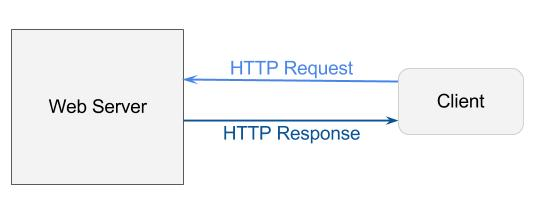
\includegraphics{img/web-server.jpg}}
                    \caption{Model komunikace webového serveru s~klientem \cite{webserverVsServletPage}}
                    \label{imgWebserver}
                \end{center}
            \end{figure}    %TODO fix obrazek je potreba prekreslit

        \subsection{Servlet kontejner} \label{servletKontejner}
            Jelikož dostávat stále stejná statická data při stejném požadavku není dostatečná funkcionalita serveru,
            tak existují způsoby jak zajistit dynamickou práci s~daty na serveru a~tudíž i~poskytovat
            měnící se odpovědi na stejný dotaz.
            Jedním ze způsobů jak této funkce docílit je využití tzv. \emph{servletů},
            které jsou navrženy pro programovací jazyk Java.

            Servlet je standardní program (konkrétně jedna třída) napsaný v~jazyce Java, 
            který implementuje rozhraní \texttt{javax.servlet}.
            Implementace tohoto rozhraní ho zavazuje k~definování několika metod, ale jinak se jedná o~běžnou
            třídu z~které jsou při zpracovávání požadavků vytvářeny její instance. Po obdržení nějakého
            požadavku provádí zpracování vstupních dat a~následně odeslání patřičné odpovědi.

            Základní myšlenkou servlet kontejneru je umožnit dynamicky vytvářet odpovědi (často webové stránky)
            pomocí vykonávání servletů. Samotný servlet kontejner je program, který poskytuje běhové prostředí pro vykonávání servletů,
            zajišťuje jejich vytváření, vykonávání a~odstraňování. Dále se také podílí na zpracovávání příchozích požadavků, které jsou
            mu předávány od webového serveru. 

            Popsaný způsob fungování servlet kontejneru je znázorněn na obrázku \ref{imgServlet}.
            %teoreticky bych mohl dopsat něco o způsobu vyhodnocení servletu, ale to asi není podstatné
            \begin{figure}[ht]
                \begin{center}
                    \scalebox{0.75}{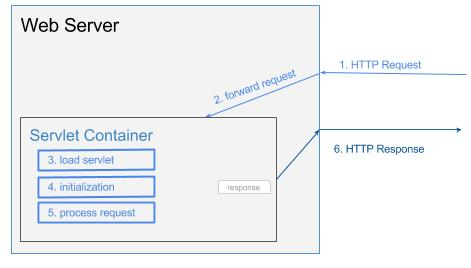
\includegraphics{img/servlet-container-life-cycle.jpg}}
                    \caption{Ukázka způsobu činnosti servlet kontejneru a~jeho spolupráce s~webovým serverem \cite{webserverVsServletPage}}
                    \label{imgServlet}
                \end{center}
            \end{figure}   %TODO fix obrazek je potreba prekreslit

        \subsection{Architektura archivu webové aplikace}
            %TODO Pridat něco o webových aplikacích, souboru web.xml, archivu .war?


         
    %%%%%%%%%%%%%%%%%%%%%%%%%%%%%%%%%%%%%%%%%%%%%%%%%%%%%%%%%%%%%%%%%%%%%%%%%%%%%%%%%%%%%%%%%%%%%%%
    \section{Nástroj Maven} \label{maven}
         %TODO zkontrolovat, jestli to dává smysl a není to moc rozvláčné
        Pro vývoj a práci se serverem Jenkins CI v podobě zdrojových kódů je zapotřebí nástroj Maven. 
        Jeho využití je také nutné při vytváření programu, který provede integraci serveru Undertow do Jenkins CI. 
        V této kapitole budou o něm poskytnuty základní informace. Pro případné bližší
        seznámení s tímto nástrojem lze další informace získat z webových stránek projektu \cite{mavenWeb}
        z kterých byly čerpány informace v této kapitole. 
        
        Maven je nástroj, který provádí činnosti spojené s vytváření spustitelných aplikací ze zdrojových kódů 
        Je zaměřen na aplikace vytvářené v jazyce Java. Hlavním cílem je umožnit uživatelům v co nejkratším
        čase provádět běžné a opakující se úkony při překladu aplikace. Především umožňuje
        provádění překladu aplikací, jejich spouštění automatizovaných jednotkových a 
        integračních testů, uložení spustitelné podoby aplikace do lokálního repozitáře 
        a případně i nahrání vytvořené aplikace na nějaký server. 

        Je dodáván jako aplikace, která se spouští z příkazové řádky příkazem \texttt{mvn}. Veškeré
        informace o projektu a definice činnosti, které má Maven provést, se specifikuje 
        v XML souboru \texttt{pom.xml}. Mezi nejdůležitější patří definice výsledné podoby aplikace
        a způsob jejího překladu, informace o závislostech
        projektu na jiných knihovnách a definice serverů z kterých má stahovat potřebné knihovny pro svůj 
        běh i pro běh aplikace. Po spuštění aplikace jsou tedy lokalizovány knihovny na kterých projekt
        závisí a uloženy v lokálním repozitáři aniž by se o tuto činnost uživatel musel dále starat.
        Kromě těchto praktických činností také umožňuje zveřejnit podrobnější informace o projektu         
        jako jsou informace o licenci, vývojářích, adrese systému pro správu verzí, atp.


        Na příkladu \ref{jenkinsPom} je ukázka části souboru \texttt{pom.xml}, který je vytvořen pro Jenkins~CI:
        \begin{priklad} \label{jenkinsPom} 
            Ukázka souboru \texttt{pom.xml}
\begin{verbatim}
  ...
  <repositories>
    <repository>
      <id>repo.jenkins-ci.org</id>
      <url>http://repo.jenkins-ci.org/public/</url>
  ...
  <dependency>
    <groupId>org.mockito</groupId>
    <artifactId>mockito-core</artifactId>
    <version>1.8.5</version>
  </dependency>
  ...
\end{verbatim}
        \end{priklad}

        V části \texttt{repository} je definována cesta k serveru z kterého má Maven stahovat potřebné soubory
        a v těle značky \texttt{dependency} je pomocí hodnot \texttt{groupId, artifactId, version} jednoznačně
        definována potřebná knihovna. Na základě těchto informací poté Maven při překladu stáhne požadovanou
        knihovnu a při distribuci aplikace nemusí být tato knihovna k programu přibalena. 


    %%%%%%%%%%%%%%%%%%%%%%%%%%%%%%%%%%%%%%%%%%%%%%%%%%%%%%%%%%%%%%%%%%%%%%%%%%%%%%%%%%%%%%%%%%%%%%%
    \section{Server Jetty} \label{jetty}
        Jednou z~komponent, které jsou aktuálně integrovány do serveru Jenkins CI, je webový server Jetty.
        Tento server je open source projektem vyvíjeným pod licencemi 
        Eclipse\footnote{Licence Eclipse je dostupná na adrese \texttt{http://www.eclipse.org/legal/epl-v10.html}}
    a~Apache\footnote{Licence Apache je dostupná 
        na adrese \texttt{http://www.apache.org/licenses/LICENSE-2.0.html}}. 
            Je využíván velkým množstvím nástrojů jako jsou například \emph{Eclipse IDE}\footnote{Webové stránky nástroje Eclipse IDE 
        \texttt{http://www.eclipse.org/}} nebo \emph{Google AppEngine}\footnote{Webové stránky platformy Google AppEngine
        \texttt{https://developers.google.com/appengine/}}.

        Jetty je webový server a~poskytuje funkcionalitu servlet kontejneru dle specifikace verze 3.0. 
        Je jej možné využít také jako webového klienta pro komunikaci se servery. Komunikace
        klientů i~serverů využívajících Jetty probíhá asynchronně. 
        Návrh serveru umožňuje samostatné spouštění aplikací i~jeho integraci do jiné aplikace. 

        %TODO nějaké reference na ty tachnologie, možná popsat SPDY a AJP13
        Kromě těchto základních možností obsahuje
        řadu souvisejících technologií jako jsou SPDY, webové sokety\footnote{Oficiální stránky 
            specifikace webových soketů: \texttt{http://www.websocket.org/}}(angl. \emph{websocket}),
        JNDI, OSGi, JMX a~další. 
        Informace v~této kapitole byly čerpány z~webových stránek serveru Jetty \cite{jettyWeb}, kde lze nalézt 
        další informace o~zmíněných technologiích a~o~tomto serveru.
        
        Aktuální využití serveru Jetty v~aplikaci Jenkins CI je podrobněji rozebráno
        v~kapitole~\ref{vyvojWinstone} a~jeho srovnáním se serverem Undertow se 
        zabývá kapitola \ref{srovnani}.
        

    %%%%%%%%%%%%%%%%%%%%%%%%%%%%%%%%%%%%%%%%%%%%%%%%%%%%%%%%%%%%%%%%%%%%%%%%%%%%%%%%%%%%%%%%%%%%%%%
    \section{Servlet kontejner Winstone} \label{winstone}
        Další komponentou serveru Jenkins CI je servlet kontejner Winstone.
        Winstone je velmi jednoduchý a~poskytuje funkcionalitu
        servlet kontejneru aniž by byl zatížen velkým množstvím požadavků, které jsou ve specifikaci jazyka Java EE.
        Nikdy neposkytoval veškeré služby servlet kontejneru, které specifikace jazyka definuje. 
        V~jeho názvu je zahrnutý pouze pojem servlet kontejner, ale tato aplikace vykonává i~služby
        webového serveru odpovídající popisu v~kapitole \ref{servletWebserver}.

        Hlavními cíli projektu bylo poskytovat funkcionalitu servlet kontejneru pouze pro jednu aplikaci,
        což je opačný přístup než u~běžných aplikačních serverů jako jsou Glasfish, JBoss, aj.
        Díky jeho omezeným službám je jeho velikost velmi malá a~umožňuje jednoduchou integraci
        s~cílovou aplikací.

        Uvedené informace byly čerpány z~oficiální stránky projektu Winstone \cite{winstoneWeb}.

        \subsection{Nedostatky servlet kontejneru Winstone}
            Původní myšlenka jednoduchého servlet kontejneru byla pro projekt Jenkins CI zajímavá, ale
            kontejner Winstone má několik zásadních nedostatků kvůli kterým bylo časem jeho využití
            v~Jenkins CI problematické \cite{kohsukeTopic}. 

            Vývoj projektu Winstone již před delší dobou ustal a~tím pádem nebyla poskytována 
            žádná další podpora pro řešení a~opravování objevených nedostatků a~chyb. 
            Značné množství bezpečnostních chyb objevených v~projektu Jenkins CI bylo právě
            způsobeno tímto servlet kontejnerem.

            Zpočátku možnosti servlet kontejneru postačovaly, ale časem je potřeba, aby 
            byly přidávány nové funkcionality, které odpovídají aktuálním trendům
            a~novým specifikacím. Příkladem mohou být nové specifikace servlet kontejneru nebo
            vývoj nových technologií jako webové sokety.


    %%%%%%%%%%%%%%%%%%%%%%%%%%%%%%%%%%%%%%%%%%%%%%%%%%%%%%%%%%%%%%%%%%%%%%%%%%%%%%%%%%%%%%%%%%%%%%%
    \section{Vývoj servlet kontejneru v~komunitě Jenkins CI} \label{vyvojWinstone}
        Po ukončení vývoje projektu Winstone se musela o~jeho potřebné úpravy starat komunita
        Jenkins CI. Takováto práce je pro komunitu velmi zatěžující
        a~naprosto neefektivní. Byly prováděny především nutné opravy bezpečnostních chyb v~kontejneru,
        ale jinak aplikace dále degenerovala. Pro tento vývoj vznikl v~projektu Jenkins CI nový 
        repozitář, který vycházel z~původní verze servlet kontejneru 
        Winstone\footnote{Repozitář, kde komunita Jenkins CI provádí úpravy projektu Winstone:
        \texttt{https://github.com/jenkinsci/winstone}}. Z~tohoto zdroje
        a~z~článku o~integraci Jetty s~kontejnerem Winstone \cite{kohsukeTopic} jsou čerpány uváděné informace. 
        
        \medskip
        Vývoj původního servlet kontejneru Winstone probíhal uvedeným způsobem 
        až do verze \emph{0.9.10-jenkins-47}. Následně byl tento způsob vývoje zastaven
        a~do kontejneru Winstone byl integrován webový server a~servlet kontejner
        Jetty. Tímto krokem vznikla 
        interní verze servlet kontejneru \emph{Winstone 2.0}. Velká část kódu 
        kontejneru Winstone byla odstraněna a~veškerá činnost webového serveru a~servlet 
        kontejneru je nyní vykonávána pomocí serveru Jetty. Z~původního kontejneru Winstone
        zůstal způsob zpracovávání a~nastavování parametrů. 
        Tato změna proběhla poměrně narychlo
        a~nebyla detailně otestována. Obsahuje zřejmě ještě množství nepotřebného kódu
        a~samotná implementace je dosti nepřehledná.

        
        %%%%%%%%%%%%%% TODO DŮLEŽITÉ KONTROLOVAT SMYSL %%%%%%%%%%%%%%%%%%%%
        \medskip
        Těsně před integrací serveru Jetty s~Jenkins CI
        vznikalo zadání tohoto diplomového projektu, které mělo za cíl
        výrazně zlepšit aktuální stav servlet kontejneru v~projektu Jenkins~CI. Během
        formulace zadání byl servlet kontejner v~projektu přepracován a~proto
        muselo být zadání upraveno. I~po této změně byly stále důvody pro 
        nahrazení stávajícího servlet kontejneru serverem Undertow.
        Aktuální situace již není tak kritická jako v~předchozí verzi,
        ale může přinést ještě další zlepšení.
                

    %%%%%%%%%%%%%%%%%%%%%%%%%%%%%%%%%%%%%%%%%%%%%%%%%%%%%%%%%%%%%%%%%%%%%%%%%%%%%%%%%%%%%%%%%%%%%%%
    \section{Server Undertow} \label{undertow}
        Undertow je webový server napsaný v jazyce Java, 
        který vzniká za podpory firmy Red Hat a~její sekce JBoss.
        Primárním účelem serveru Undertow je být výchozím webovým serverem v~aplikačním serveru WildFly.
        Jeho první verze finální byla vydána teprve před nedávnem, takže se jedná o
        nově vytvořený server a jeho vývoj stále usilovně 
        probíhá\footnote{Aktuální verzi serveru, lze najít na serveru GitHub: 
        \texttt{https://github.com/undertow-io/undertow}}. Pro stažení a využití tohoto serveru
        je nejjednodušší využít aplikaci Maven (kapitola \ref{maven}) a nastavit patřičnou 
        závislost\footnote{Definice závilosti v aplikaci Maven pro stažení serveru Undertow: 
        \texttt{http://undertow.io/downloads.html} }.

        Informace v~této kapitole byly čerpány především z~webových stránek projektu \cite{undertowWeb} a 
        jeho dokumentace \cite{undertowDocs},
        ale jelikož je aplikace poměrně nová, tak zveřejněná dokumentace je poměrně nedostatečná. 
        Některé informace z~této kapitoly musely být čerpány
        z~vygenerované projektové dokumentace a z komunikace s vývojáři projektu
        na chatu IRC.

        \subsection{Vlastnosti serveru}
            Server Undertow je zaměřen na to, aby byl plně integrovatelný do libovolných aplikací
            a~byl co nejmenší a~nejjednodušší. Samotný
            archiv s~jádrem aplikace je menší než 1MB a~při běhu aplikace potřebuje
            méně než 4MB dynamicky alokované paměti. 

            Je navržen takovým způsobem, aby při implementaci mohl uživatel využít
            jen část aplikace, kterou nutně potřebuje, a~patřičně si ji upravit
            pro své vlastní potřeby.
            Tohoto přístupu je dosaženo kombinováním a~řetězením
            obslužných funkcí (angl. \emph{handler}), které server poskytuje.
            Díky tomuto přístupu je server velmi flexibilní a~v~jeho důsledku
            také patřičně rychlý, protože uživatele nebrzdí funkcionality
            serveru, které nutně nepotřebuje a~nevyužívá.
            
            Při komunikaci umožňuje server podporu jak pro asynchronní, tak
            pro synchronní komunikaci.
            Dalšími funcionalitami, které server poskytuje, jsou možnost integrace
            servlet kontejneru odpovídajícího specifikaci verze 3.1,
            využití plné podpory webových soketů (angl. \emph{websockets}) nebo 
            podpory technologie \emph{HTTP upgrade}.

        \subsection{Architektura serveru}
            V této kapitole jsou podrobněji rozebrány základní principy, jak Undertow funguje, 
            a je zjednodušeně popsána jeho architektura z pohledu uživatele. Další podrobnější informace o serveru 
            lze nalézt na webové dokumentaci projektu, která byla hlavním zdrojem této kapitoly \cite{undertowDocs}.
            Popis architektury serveru se přímo vzahuje k samotné integraci do Jenkins CI.

            \subsubsection{Webový server}
                Architektura serveru Undertow nevyužívá koncept jednoho velkého kontejneru, který se pomocí vysokoúrovňového rozhraní nastaví 
                pro danou aplikaci a sám o sobě funguje. Naopak aplikace jsou sestavovány z množství tříd tzv. \emph{handlerů} 
                (viz níže), které spravují příchozí požadavky a samy o sobě utvářejí samotný webový server. 
                Díky tomuto konceptu je možné využít jen tu funkcionalitu serveru, která je v aplikaci potřeba, a server
                není brzděn zbytečnou činností, která není pro konkrétní aplikaci potřebná. 

                Vstupním bodem aplikace jsou tzv. \textbf{\emph{listenery}} (angl. \emph{listener}), které naslouchají na určených síťových
                rozhraních a portech a zpracovávají příchozí požadavky. Jednotlivé \emph{listenery} se liší dle protokolu, kterým komunikují.
                V Undertow jsou 3 základní typy \emph{listenerů}
                pro protokoly HTTP, HTTPS, a AJP. Také je vytvořen podpora protokolu SPDY, ale v aktuální verzi ještě není zahrnuta. 
                Pro uživatele poskytují abstrakci nad samotnými síťovými protokoly, takže v serveru lze stejným způsobem zpracovávat
                požadavky přicházejícími v různých protokolech. Jediným samozřejmým omezením je, že nelze v jednom protokolu
                používat informace specifické pouze pro protokol jiný. 
                
                Pro umožnění této abstrakce každý \emph{listener} provádí překlad 
                požadavku do objektu třídy
                \texttt{HttpServerExchange}. V něm je uchováván aktuální stav požadavku a vytvářené odpovědi
                a při odesílání odpovědi z tohoto objektu \emph{listener} vytvoří odpověď, která je poslána klientovi.

                Tyto listenery jsou těsně navázané na knihovnu XNIO\footnote{TODO}, která
                poskytuje pro Undertow abstrakci nad síťovou komunikací. Samotné listenery v Undertow je možné konfigurovat
                nastavením několika parametrů \cite{undertowListeners}, ale lze také přímo konfigurovat síťové kanály knihovny XNIO.

                \medskip
                Samotné jádro serveru tvoří již zmiňované \emph{handlery}.
                \textbf{\emph{Handler}} je třída, která definuje metodu \texttt{handleRequest} v níž
                je příchozí požadavek na serveru libovolně upraven a předán dalšímu \emph{handleru} ke zpracování nebo je vytvořena odpověď 
                a poslána zpět klientovi (tedy jsou vynechány následující \emph{handlery}). 
                \emph{Handlery} jsou tedy za sebou napojeny a tvoří řetěz (angl. \emph{handler chain}).
                Je možné si nadefinovat libovolný vlastní \emph{handler}, který pouze musí implementovat patřičné rozhraní s metodou 
                \texttt{handleRequest} nebo je možné využít již předpřipravených tříd. V těchoto předpřipravených třídách
                jsou běžně požadované funkce serveru jako úprava hlaviček příchozího požadavku, přesměrování požadavku apod.
                Pomocí jediného parametru (objekt třídy \texttt{HttpServerExchange}) metody \texttt{handleRequest} 
                si \emph{handlery} předávají aktuální stav požadavku a postupně vytvářené odpovědi.


                Popisované \emph{handlery} a \emph{listenery} jsou základem architektury serveru Undertow, terá je znázorněna
                na obrázku \ref{imgUndertowArchitecture}. 
                Na příkladu \ref{prUndertow} je ukázáno vytvoření jednoduchého webového serveru.

                \begin{figure}[ht]
                    \begin{center}
                        \scalebox{0.63}{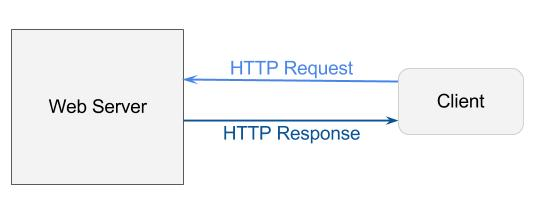
\includegraphics{img/web-server.jpg}}
                        \caption{Architektura serveru Undertow}
                        \label{imgUndertowArchitecture}
                    \end{center}
                \end{figure}    %TODO fix obrazek je potreba nakreslit
  


                %TODO kontrola posunutí textu
                \newpage
\begin{priklad} \label{prUndertow} Vytvoření jednoduché instance serveru Undertow
\begin{verbatim}
Undertow server = Undertow.builder()
  .addHttpListener(8080, "localhost")
  .setHandler(new HttpHandler() {
    @Override
    public void handleRequest(final HttpServerExchange exchange) 
        throws Exception {
      exchange.getResponseHeaders().put(Headers.CONTENT_TYPE, "text/plain");
      exchange.getResponseSender().send("Hello World");
    }
  }).build();
server.start();
\end{verbatim}
\end{priklad}

                
            Třída \texttt{Undertow} reprezentuje instanci samotného
            webového serveru a~je ji nutné definovat prakticky vždy. Metodou
            \texttt{addListener} je přidán výše zmiňovaný \emph{listener}, který
            naslouchá na zvoleném síťovém rozhraní a portu (při zvolení IP adresy 0.0.0.0 naslouchá
            na všech rozhraních). Tento jednoduchý příklad obsahuje pouze jeden \emph{handler} 
            přidaný metodou \texttt{addHandler}, který
            provádí veškerou činnost serveru a tou je odpovídání na všechny požadavky jednotným textem. 
            Ve standardních aplikacích by následovalo volání dalšího \emph{handleru}.

            \subsubsection{Integrace servlet kontejneru}
                %Vytvoření DeploymentInfo a nastavení požadovaných funkcí 
                %infastuktury servlet kontejneru.
                %vytvoreni veci z web.xml

                %Vhodné využití statických metod z io.undertow.servlets.Servlets
                %Správa statických zdrojů pomocí ResourceManager.

                %Ukázka vytvoreni deployment info

            \subsubsection{Zabezpečení servlet kontejneru}
                %Nastavení autentizace pomocí LoginConfig, IdentityManageru, 
                %security-constraints z web.xml
                
 
        
        \subsection{Srovnání serverů Undertow a~Jetty}\label{srovnani}
            Stávající servlet kontejner v~Jenkins CI je sice tvořen
            kombinací kontejneru Winstone a~serveru Jetty, ale veškerou
            časově kriticky náročnou práci při běhu aplikace vykonává server
            Jetty. Proto pokud chceme srovnávat původní a plánované řešení servlet kontejneru
            v~Jenkins CI, tak bychom měli srovnávat server Jetty se serverem Undertow.

            \medskip
            Budeme tedy srovnávat servery Undertow a~Jetty, jejich výhody a~nevýhody
            vzhledem k~využití v~systému Jenkins CI:
            \begin{itemize}
                \item {\textbf{Rychlost:} Server Undertow je sice nový, ale už přesto existují
                    testy v~kterých se ukázal být výkonnější než server Jetty. V~tomto           
                    testování\footnote{Porovnání rychlosti, odezvy a~celkové výkonnosti serverů Undertow, Jetty a~jiných: 
                    \\\texttt{http://www.techempower.com/benchmarks/\#section=data-r8\&hw=ec2\&test=plaintext}}
                    byl server Undertow v některých případech byl server 
                    Undertow i~3,5 krát rychlejší než server Jetty v~počtu zpracovaných 
                    požadavků za jednotku času. Při porovnávání doby odezvy serveru na požadavek 
                    dosáhl server Undertow až třetinového času než server Jetty. 
                    
                    Naopak při některých
                    jiných konfiguracích byl server Jetty rychlejší a proto nelze definitivně určit,
                    který server je rychlejší a podstatné je také způsob využití serveru. 
                    Dalším důležitým faktem je, že v Jenkins CI není využita nejnovější verze serveru
                    Jetty (verze 9), ale jeho nižší verze 8, protože Jenkins CI aktuálně využívá
                    starší verzi jazyka Java (verzi Java 6).
                    
                    Lze tedy usuzovat, že server Undertow má potenciál být výkonnějším.
        
                    V rámci této práce bylo provedeno vlastní základní testování 
                    obou těch serverů a to ve vztahu přímo k systému Jenkins CI. Tímto testováním
                    se zabýcá kapitola \ref{kapPerformance}, kde jsou porovnávány 
                    implementace servlet kontejneru s využitím serveru Jetty a nové implementace 
                    postavené na serveru Undertow.
                    }

                \item{\textbf{Spolehlivost:} Dalším důležitým aspektem je spolehlivost daného serveru. 
                        Server Jetty má za sebou již dlouhou historii a~je integrován ve velkém množství
                        různých aplikací\footnote{Aplikace, které využívají server Jetty: \texttt{http://www.eclipse.org/jetty/powered/}},
                        což mu dodává velkou důvěryhodnost a~lze očekávat, že bude pracovat velmi 
                        spolehlivě. 
                        
                        U~serveru Undertow byla dokončena první finální verze teprve nedávno,
                        takže lze předpokládat, že může obsahovat ještě drobné nedostatky,
                        které budou časem opravovány. Jelikož tento server je integrován
                        v~novém aplikačním serveru WildFly 8, tak lze předpokládat,
                        že postupem času bude také velmi spolehlivý. 
                        Nicméně v~tomto aspektu je server Jetty zřejmě 
                        aktuálně lepší.}

                \item{\textbf{Rychlost spuštění:}  Velmi často je u~serverů hodnocena hlavně
                    jejich rychlost a~výkonnost v~zátěži. Je běžné, že nebývá kladen důraz na
                    velmi rychlé spuštění serveru. Pro standardní běh serveru, kdy bývá 
                    spuštěn jednou za několik týdnů či měsíců po nějakých úpravám aplikace,
                    není doba spuštění zásadní. Pokud se na to podíváme z~pohledu testování
                    aplikace, kdy jsou spouštěny integrační testy a~pro každý test musí být
                    znovu spuštěn server, tak je rychlost nastartování serveru velmi podstatná.
                    
                    Cílem serveru Undertow je být minimalistickým a~velmi rychlým 
                    řešením. Server Jetty poskytuje kvalitní podporu pro běh aplikací, ale je 
                    rozsáhlejší. 
                    Lze usuzovat, že rychlost spuštění bude u~serveru Undertow výrazně nižší
                    než u~serveru Jetty. 
                    
                    %TODO potřeba zvážit, ale spíše to není podstatné
                    %Tato skutečnost bude testována při vyhodnocování
                    %výsledků této diplomové práce.

                    V~aktuálním stavu Jenkins CI běží integrační testy více než hodinu. Pokud 
                    by byl servlet kontejner spuštěn za výrazně kratší dobu, tak by mohla být doba testování
                     také výrazně zkrácena. 
                    }

                \item{\textbf{Velikost:} Jelikož je servlet kontejner přímo integrován do archivu ve kterém
                    je systém Jenkins CI distribuován, tak komunita dbá na to, aby přidávané komponenty
                    nebyly příliš velké a~průběžně sleduje aktuální velikost
                    výsledného archivu\footnote{Stránka, kde je v~systému Jenkins CI automatizovaně
                    sledována velikost archivu aplikace:\\ 
                    \texttt{https://wiki.jenkins-ci.org/display/JENKINS/Jenkins+WAR+Size+Tracker}}.  
                                       
                    Po integraci Jetty vzrostla velikost servlet kontejneru o~1,5 MB na celkovou
                    velikost 1,8 MB. U~serveru Undertow je uváděno, že jeho archiv má méně
                    než 1 MB, ale~konečná velikost po integraci bude také záležet na využitých komponentách
                    a~rozsahu implementace. Přesto z~pohledu velikosti výsledného archivu
                    se jeví server Undertow jako výhodnější, ale rozdíl oproti serveru Jetty není zásadní.}

                %Tato část by měla být pečlivě překontrolována
                \item{\textbf{Konfigurovatelnost:} Server Undertow je velmi flexibilní a~způsob
                    jeho návrhu, který byl popsán výše, umožňuje provádět mnoho různých úpravy 
                    své činnosti dle potřeby a~využít pouze ty části, které potřebujeme.
                    Tato filozofie je velmi blízká filozofii projektu Jenkins CI. 
                    
                    Server Jetty
                    je oproti tomu robustnější a~rozsáhlejší, ale neumožňuje tak velké přizpůsobování potřebám
                    uživatele jako například využití jen několika malých částí jeho funkčnosti či jejich
                    kombinování. }


                \item{\textbf{Snadnost použití:}}                      
                    Server Jetty má již dlouhou historii a je v něm vše pečlivě dokumentováno
                    a to jeho využití pro uživatele činí poměrně snadným. Podstatnou výhodou je, že
                    server Jetty poskytuje velké množství vysokoúrovňových rozhraní
                    pro různé konfigurace serveru.
                    
                    Jelikož je server Undertow velmi mladým projektem a není tolik ustálený, 
                    tak postrádá některé věci,
                    které jsou u serveru Jetty samozřejmostí. 
                    Dokumentace k serveru
                    Undertow je poměrně strohá, místy ne úplně přesná a stále se vyvíjí. 
                    Jeho velká flexibilita při konfiguraci s sebou nese i jisté nevýhody
                    a tím je právě jednoduchost jeho použití. Další nepříjemností je, že není
                    dostupné tolik propracované rozhraní pro konfiguraci jako u serveru Jetty,
                    což lze opět přičítat délce trvání projektu.

                    Je zjevné, že využití serveru Jetty je podstatně jednodušší než je tomu
                    u serveru Undertow. Nicméně tato skutečnost je jen překážkou pro provedení
                    integrace, ale následně nemusí činit další problémy a nijak neovlivňuje
                    funkčnost výsledné aplikace.

            \end{itemize}
        

%%%%%%%%%%%%%%%%%%%%%%%%%%%%%%%%%%%%%%%%%%%%%%%%%%%%%%%%%%%%%%%%%%%%%%%%%%%%%%%%%%%%%%%%%%%%%%%

%%%%%%%%%%%%%%%%%%%%%%%%%%%%%%%%%%%%%%%%%%%%%%%%%%%%%%%%%%%%%%%%%%%%%%%%%%%%%%%%%%%%%%%%%%%%%%%
\chapter{Analýza současného stavu servlet kontejneru a~návrh integrace}
    Tato kapitola se zabývá důkladnější analýzou a~zkoumáním architektury aplikace Jenkins~CI
    z~pohledu jejího vestavěného kontejneru a~jeho možných úprav (kapitola \ref{secArchitecture}). 
    V~další části jsou konkretizovány jednotlivé činnosti, které současný servlet kontejner provádí
    a~které musí nová implementace také poskytovat (kapitola \ref{secKompatibilita}).
    Poslední část této kapitoly diskutuje možné varianty integrace serveru Undertow do Jenkins CI,
    jejich výhody a~nevýhody (kapitola \ref{secNavrh}). Jako výstup této analýzy je zvolen způsob integrace, který bude
    následně implementován.

    Jelikož k~této problematice je minimum oficiální zdrojů, které by danou problematiku blíže popisovaly, 
    tak podstatná část zde uváděných informací byla čerpána přímo ze zdrojových kódů aplikace a~komponent Jenkins CI.
    
    \section{Aktuální stav architektury servlet kontejneru v~Jenkins~CI}\label{secArchitecture}
        V~následujících dvou podkapitolách bude blíže analyzována architektura
        Jenkins CI z~pohledu servlet kontejneru. Tato analýza je velmi důležitá
        pro pochopení návazností jednotlivých komponent, které budou později upravovány.

        Jak již bylo uvedeno v~kapitole \ref{vyvojWinstone}, současný servlet kontejner 
        v~Jenkins CI se skládá z~nástojů Winstone a~Jetty, které byly také popisovány
        v~předchozích kapitolách. Velká část servlet
        kontejneru Winstone byla odstraněna a~zůstala pouze část, která
        provádí zpracování parametrů
        programu po spuštění aplikace. Činnost webového serveru, servlet kontejneru
        a~další vykonává server Jetty.
        

        \subsection{Architektura Jenkins CI z~pohledu servlet kontejneru} 
            Na vysoké úrovni pohledu lze architekturu serveru Jenkins CI rozdělit do tří částí:
            
            \begin{itemize}
                \item{\textbf{Jádro aplikace} do kterého patří nejnutnější základní komponenty systému a
                    části, které jsou pro Jenkins CI specifické a~vznikají v~rámci tohoto projektu.}

                \item{\textbf{Přídavné moduly} aplikace, které jsou do ní dynamicky přidávány jako archivy javových programů
                    \texttt{.jar}. Tyto součásti jsou většinou nutné pro standardní běh aplikace a~je s~nimi aplikace
                    běžně dodávána (teoreticky lze
                    aplikaci spustit např. bez servlet kontejneru pomocí aplikačního serveru, ale toto je spíše ojedinělý případ). 
                    
                    Komponenty z~této kategorie pocházejí typicky z~externích projektů.
                    Do této kategorie také spadá servlet kontejner, který je aktuálně do aplikace
                    přidáván pod názvem \texttt{winstone.jar}.}

                \item{\textbf{Rozšiřující moduly} (angl. plugins) jsou samostatné menší programy, které nějakým
                    způsobem přidávají funkcionalitu serveru Jenkins CI. Typicky nejsou dodávány s~aplikací
                    a~uživatel si je může stáhnout nebo si nějaký vlastní modul vytvořit.
                    
                    Samotná aplikace se dodává jen s~těmi nejnutnějšími součástmi a~ponechává na uživatelích, které
                    další funkcionality si do systému doinstalují. V~současné době již existují stovky takových
                    modulů, které jsou volně ke stažení. }
            \end{itemize}
            

            V~následujícím textu bude při popisu interních součástí zdrojových kódů použita notace
            ve tvaru \texttt{Název\_třídy::Název\_metody}.

            Architektura Jenkins CI z~pohledu servlet kontejneru je znázorněna na obrázku \ref{imgArchitekturaServlet}.
            Jsou zde zachyceny především komponenty, které přímo souvisejí s~jeho činností.

            \begin{figure}[h!t]
                \begin{center}
                    \scalebox{0.7}{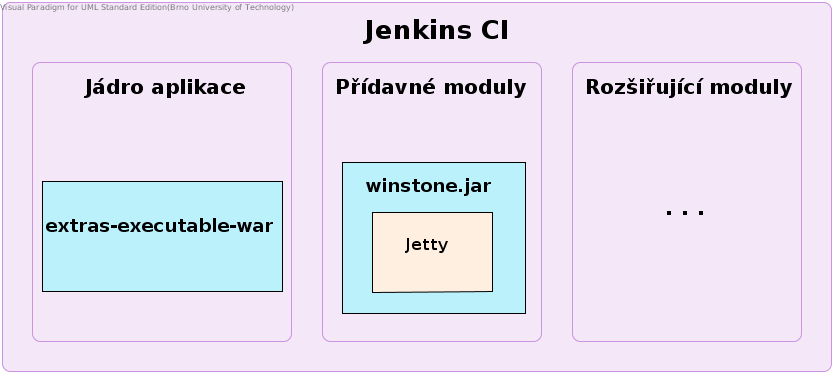
\includegraphics{img/architecture.png}}
                    \caption{Přehled architektury systému Jenkins CI z~pohledu vestavěného servlet kontejneru}
                    \label{imgArchitekturaServlet}
                \end{center}
            \end{figure}

            
            Archiv \texttt{winstone.jar} obsahuje servlet kontejner pro Jenkins CI. Název je nyní sice mírně matoucí
            (způsoben předchozí implementací), ale aktuálně jsou součástí tohoto archivu komponenty Winstone a~Jetty.

            Velmi podstatnu součásti aplikace z~pohledu servlet kontejneru je komponenta\\\texttt{extras-executable-war}. 
            Tato součást aplikace je sice malá, ale obsahuje metodu \texttt{main}, kterou se aplikace spouští 
            (pokud není spuštěna v~aplikačním serveru). Hlavním úkolem této komponenty je právě spustit 
            servlet kontejner a~tím spustit i~celou aplikaci. Tento proces spuštění aplikace je zobrazen
            na obrázku \ref{imgArchitekturaSpusteni}.

            Nejprve je spuštěna vstupní metoda celé aplikace \texttt{Main.java::main} z~komponenty\\\texttt{extras-executable-war}.
            Po počáteční inicializaci je předáno řízení aplikace metodě \\\texttt{Launcher.java::main}
            z~archivu \texttt{winstone.jar}, která provede nastartování
            a~zavedení servlet kontejneru. Následně je provedena inicializace a~spuštění
            jediného servletu aplikace Jenkins CI a~tím je servlet Stapler (bližší informace o~tomto
            servletu jsou v~kapitole \ref{secJenkinsArchitektura}). 
            Pokud se podaří úspěšně spustit tento servlet, tak je spuštění celé aplikace Jenkins CI z~pohledu
            servlet kontejneru úspěšně provedené a~aplikace běží.

            Zjištění, které komponenty má servlet kontejner při svém startu zavést,
            se nachází v~souboru \texttt{web.xml}, což je standardní konfigurační soubor
            pro webové aplikace v~jazyce Java~EE. Může se zde nacházet také
            konfigurace uživatelských účtů pro přístup k~aplikaci a~specifikování
            různých druhů přístupových práv.


            \begin{figure}[h!t]
                \begin{center}
                    \scalebox{0.64}{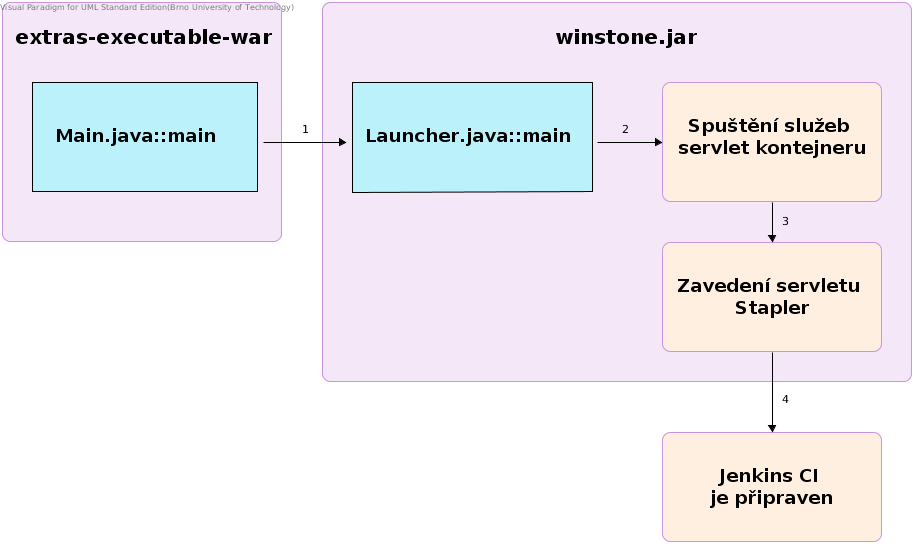
\includegraphics{img/jenkinsStart.png}}
                    \caption{Průběh spouštění aplikace Jekins CI při spouštění pomocí vestavěného servlet kontejneru}
                    \label{imgArchitekturaSpusteni}
                \end{center}
            \end{figure}


        \subsection{Průběh komunikace prostřednictvím servlet kontejneru}
            Po úspěšném zavedení a~spuštění aplikace provádí servlet kontejner
            zpracovávání příchozích požadavků a~předává je aplikaci Jenkins CI. 
            Typický zjednodušený průběh komunikace servlet kontejneru s~aplikací je znázorněn
            na obrázku \ref{imgKomunikace}. 

            \begin{figure}[h!t]
                \begin{center}
                    \scalebox{0.64}{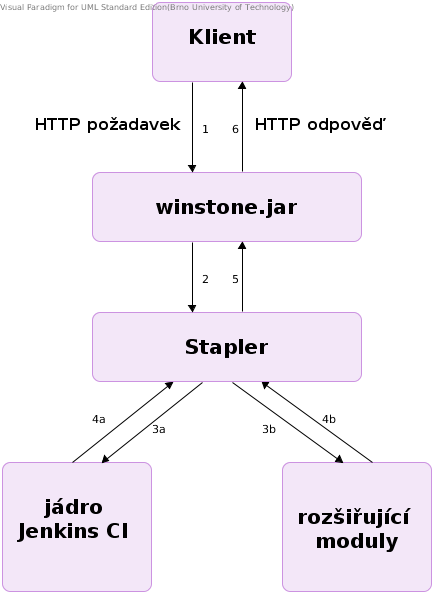
\includegraphics{img/jenkinsCommunication.png}}
                    \caption{Průběh komunikace aplikace Jekins CI prostřednictvím vestavěného servlet kontejneru}
                    \label{imgKomunikace}
                \end{center}
            \end{figure}

            Při komunikaci je příchozí HTTP požadavek zpracován pomocí servlet kontejneru 
            a~následně předán patřičnému servletu (dle nastavení pravidel pro směřování požadavků).
            Jelikož je v~aplikaci pouze jediný servlet Stapler, tak je požadavek předán jemu.
            Tato komponenta následně provede netriviálním způsobem rozhodnutí, které
            části aplikace předat požadavek k~vykonání  nebo zda náleží nějakému rozšiřujícímu modulu.
            Následně stejnou cestou probíhá zaslání HTTP odpovědi zpět klientovi.

            Byla zde zachycena pouze jedna z~možných činností
            servlet kontejneru a~tou je zpracovávání komunikace protokolem HTTP. 
            Další činnosti kontejneru budou rozebírány později.

 


    \section{Zpětná kompatibilita servlet kontejner v~Jenkins CI}   \label{secKompatibilita}
        V~této kapitole jsou blíže rozebírány a~analyzovány jednotlivé funkce servlet
        kontejneru v~Jenkins CI. Analýza jeho funkčnosti je zaměřena především na 
        návrh nového servlet kontejneru, který vznikne integrací serveru Undertow.
        Z~této kapitoly vyplynou hlavní požadavky, které bude potřeba řešit 
        při samotné implementaci.

        Stávající servlet kontejner je v~Jenkins CI již dlouhou dobu
        a~mnoho uživatelů a~komponent systému přímo používá jeho specifické
        parametry, které pocházejí z~kontejneru Winstone~\cite{kohsukeTopic}. Nová implementace
        tudíž musí zachovat naprosto stejný formát parametrů, aby 
        se výměnou servlet kontejneru nestala část aplikace nebo rozšiřujících modulů nefunkční.
        Také je potřeba zachovat výchozí hodnoty jednotlivých parametrů.

        \subsection{Funkcionality servlet kontejneru}
            Při spouštění aplikace je před předáním řízení aplikace servlet kontejneru
            část parametrů zpracována komponentou \texttt{extras-executable-war} (blíže 
            rozebrána v~kapitole \ref{secArchitecture}) a~zbylé parametry jsou přímo
            předány kontejneru, který podle nich nastaví svou činnost. Kompletní
            soupis parametrů, které jsou implementovatovány v~servlet kontejneru,
            je v~příloze \ref{prilohaParametry}.
            Jednotlivé parametry zde nejsou rozebírány, ale následující analýza
            se zaměřuje především na klíčové bodů funkčnosti servlet kontejneru.

            Pro zachování zpětné kompatibility musí servet kontejner v~aplikaci 
            Jenkins CI poskytovat následující funkce:
            
            \newpage
            \begin{itemize}
                \item{\textbf{Komunikaci nešifrovaným protokolem HTTP}}
                \item{\textbf{Komunikaci šifrovaným protokolem HTTPS}}
                \item{\textbf{Komunikaci protokolem AJP13}} 
                \item{\textbf{Umožnit přihlašování a~správu přístupových práv} }
                \item{\textbf{Umožnit restartování a~ukončování aplikace přes speciální port}}
                \item{\textbf{TODO: access logger, podrobnější popis činností}}
                \item{\textbf{TODO: Nastavení aplikace dle web.xml?}}
            \end{itemize}
            

            %v budoucnu by možná bylo vhodné popis protokolu AJP13 rozvést
            Protokoly HTTP a~HTTPS jsou velmi běžnými protokoly používanými pro 
            komunikaci aplikací ve webovém prostředí a~v~této práci je očekáváno, 
            že čtenář je s~němi již seznámen. Protokol AJP13 je speciálním
            typem protokolu, který se využívá především pro efektivnější komunikaci
            webového serveru a~servlet kontejneru \cite{ajp13Web}.
            
            Další činností kontejneru, kterou může vykonávat 
            je správa přístupových práv a~umožnění autentizace uživatelů. 
            Konkrétní uživatelské účty mohou být specifikovány
            při spouštění servlet kontejneru nebo načítány ze
            standardního konfiguračního
            souboru webové aplikace \texttt{web.xml}.
            %Tato problematika je blíže rozebírána v~následující kapitole \ref{secSecurityArchitecture}.


            Poslední z~hlavních funkcionalit, které nabízí servlet kontejner v~Jenkins CI
            a~je nutné ji zachovat,
            je možnost ukončit nebo restartovat aplikaci pomocí zaslání
            speciálního požadavku na zvolený port. 

            Po integraci serveru Jetty do servlet kontejneru byla přidána ještě možnost
            komunikace protokolem SPDY, ale tento protokol ještě není 
            v~Jenkins CI více využíván a~tudíž jeho implementace není zásadní.

        
        %Možnost rozšířiš informace o security architektuře     
        %\subsection{Bezpečnostní architektura v~Jenkins CI} \label{secSecurityArchitecture}
        %            \cite{securityArchitectureJenkins}, \cite{securityArchitectureWinstone}
        %            


    \section{Návrh způsobu integrace serveru Undertow} \label{secNavrh}
        Na základě analýzy, která proběhla v~předchozích kapitolách,
        je v~této kapitole zvolen způsob
        integrace serveru Undertow do systému Jenkins CI. 
        Obě navržené možné varianty integrace jsou porovnány z~různých
        hledisek a~je zvolen způsob, kterým bude následně implementace provedena.

        Na závěr kapitoly jsou popsány problémy, které byly objeny při analýze
        a~mají dopad na samotnou integraci a~její výsledky.
                
        \subsection{Varianty integrace}
            Pro integraci serveru Undertow do systému Jenkins CI jsou možné tyto dva přístupy:

            \begin{enumerate}
                \item{Nahrazení pouze serveru Jetty v~servlet kontejneru a~ponechání
                    zbytku implementace kontejneru Winstone, což by představovalo
                    pouze úpravy části stávajícího kódu. }

                \item{Nahrazení jak serveru Jetty tak kontejneru Winstone. 
                    Tento přístup v~podstatě znamená provedení celé implementace
                    servlet kontejneru pro Jenkins CI úplně znovu.}
            \end{enumerate}

            \noindent Obě varianty integrace mají své klady a~zápory. 
            Srovnáme je z~hlediska výkonu, proveditelnosti a~zpětné kompatibility
            implementace, abychom mohli následně zvolit vhodnější variantu:

            \begin{itemize}
                \item{\textbf{Srovnání výkonu:} V~první variantě integrace je ponechána stále
                 velmi stará implementace kontejneru Winstone, která zřejmě stále ještě
                 obsahuje nepotřebné součásti a~samotný způsob inicializace není optimalizován
                 pro potřeby serveru Undertow, takže by mohlo docházet ke zbytečnému
                 zpomalování aplikace.
                 Nová implementace může být přímo optimalizována pro potřeby 
                 serveru Undertow a~poskytovat lepší výkon i~kratší dobu spuštění aplikace, 
                 která není zanedbatelná při spouštění integračních testů.}

                \item{\textbf{Srovnání proveditelnosti:} První varianta představuje provedení 
                    úprav pouze v~částech, kde je přímo integrován server Jetty, 
                    zatímco v~druhé variantě je potřeba provést znovu celou implementaci
                    integrace servlet kontejneru. 
                                         
                    V~tomto případě je úprava stávajícího kódu aplikace
                    zřejmě snazším přístupem a~také umožňuje provedení rychlejší
                    implementace, protože není nutné návrhovat celý modul,
                    ale pouze jeho části.}

                \item{\textbf{Srovnání zpětné kompatibility:} Dosažení zpětné kompatibility
                    u~první varianty je snazší, jelikož jsou viditelná místa, která je 
                    potřeba znovu implementovat a~nezanedbat. Nicméně druhá varianta
                    nemá žádné faktické nevýhody k dosažení 
                    stejné úrovně zpětné kompatibility jako varianta první.}

                \item{\textbf{Další hlediska:} Jelikož dlouhodobý vývoj servlet kontejneru
                    v~Jenkins CI je na okraji zájmu a~jsou prováděny především nejnutnější úpravy, 
                    tak celý kód poněkud zdegeneroval a~je obtížně čitelný, což
                    je velká závada u~open source projektu. Tato skutečnost
                    může bránit dalším přispěvovatelům k~provádění potřebných změn.

                    Z~tohoto pohledu by nová implementace mohla přinést mnohem čitělnější
                    způsob řešení a~zbavit se zbytečností z~původní realizace servlet kontejneru.}
            \end{itemize}


            Bez ohledu na zvolený způsob integrace bude jeho výsledkem především nový archiv \texttt{.jar},
            který bude obsahovat příslušnou integraci. Pro jeho využití v~systému Jenkins CI je potřeba
            upravit několik konfigurací a~případně upravit jeho načítání při spouštění aplikace v~modulu
            \texttt{extras-executable-war}, což bylo rozebíráno v~kapitole \ref{secArchitecture}.


        \subsection{Zvolení způsobu integrace}
            Při výběru varianty integrace serveru Undertow do Jenkins CI byly zváženy
            výhody a~nevýhody, které byly popsány v~předchozí kapitole. Při nahrazení pouze serveru Jetty
            by provedení integrace zřejmě probíhalo podstatně snadněji než ve variantě druhé,
            ale z~kvalitativního pohledu se tato varianta jeví jako méně vhodná. 

            Při implementaci budou tedy nahrazeny obě komponenty stávajícího servlet kontejneru
            a~bude tudíž provedena celá implementace znovu s~využitím serveru Undertow. Tato
            varianta by měla přinést lepší čitelnost zdrojového kódu a~poskytnout 
            lepší výkonnost celé aplikace než druhá varianta.

        \subsection{Zjištěné problémy}
            Při analyzování možností integrace byly zjištěny dva problémy.

            Prvním problémem je, že server Undertow
            je určen pro běh pod virtuálním strojem, který odpovídá specifikaci jazyka
            Java verze 7, zatímco server Jenkins CI využívá verzi 6. 
            Server Jenkins CI využívá starší verzi z~důvodu zpětné kompatibility
            řešení. 
            
            Specifikace jazyka je plně zpětně kompatibilní, takže server Jenkins CI
            může být spuštěn s~novější verzí virtuálního stroje, ale pro okamžité začlenění
            serveru Undertow do Jenkins~CI je tato skutečnost problém. Pokud by ovšem
            provedená integrace poskytovala dobré výsledky, tak by bylo možné 
            upravit kód serveru Undertow tak, aby odpovídal starší specifikaci.
            V~těchto verzích jazyka není zásadní rozdíl a~úprava by byla jistě
            možná, ale velmi pracná a~stále by potřebovala údržbu při příchodu
            nových verzí serveru Undertow. Další možností je
            zvýšit tlak na přechod celé aplikace na novější verzi specifikace jazyka,
            což výhledově jistě nastane, ale není jisté kdy. 

            V~této práci bude tento problém vyřešen převedením aplikace Jenkins CI na vyšší verzi,
            což představuje úpravu několika konfigurací.

            \medskip        
            Druhým problémem je, že při integraci serveru Jetty do Jenkins CI byla přidána
            možnost využít protokol SPDY, jehož implementace
            není v~současné době v~serveru Undertow dostupná. Nicméně tato možnost
            je zavedena jen krátce a~zřejmě ještě není využívána žádnými komponentami,
            takže by neměl být problém, kdyby nová implementace neobsahovala tuto volbu.
            
            Je důležité dodat, že požadavek na implementaci 
            protokolu SPDY byl v~komunitě serveru Undertow vznesen
            a~je také zaznamenán v~systému pro sledování chyb\footnote{
                Plánovaná implementace protokolu SPDY v~serveru Undertow:
                \texttt{https://issues.jboss.org/browse/UNDERTOW-9}}.
            Je tedy možné, že tato funkcionalita bude v~blízké době době do serveru
            Undertow přidána.
            



    \section{Implementace}
%                    V mnoha místech navíc chybí patřičné komentování zdrojových kódů a to
%                    i na úrovni veřejného rozhraní, což činilo využití poměrně náročným a byl jsem nucen zkoumat
%                    samotné zdrojové kódy serveru, abych vše správně pochopil a využil.

        %web.xml - podpora určitých parametrů, ale zachování obecnosti
        %
        %využit parametr setIgnoreFlush

    \section{Srovnání výkonu původní a nové implementace}  \label{kapPerformance}
    %Různé scénáře, prootože rychlost určuje taky jak jsou rychle odpovědi servlet kontejneru na požadavky servletu
    %proto i různé stránky, ale není to jen o servlet kontejneru, ale také o tom, jak je napsán kontejner
    %
    %používá jen POST a GET, pro DELETE se dělá POST (získáno z popisu REST API /job/jobName/API)
    %Testovány nejpodstatnější části webserveru - komunikace pomocí HTTP a HTTPS




\chapter{Závěr}
    Začátek této práce se věnoval seznámení s~integračním serverem Jenkins CI,
    se servery Jetty a~Winstone, které jsou součástí jeho servlet kontejneru,
    a~se serverem Undertow, jehož integrace do Jenkins CI je hlavní
    náplní této práce. V~následující části byla analyzována architektura aplikace Jenkins CI
    a~také stav servlet kontejneru, který je v~něm integrován.

    Po seznámení se s~podmínkami pro integraci byly
    zkoumány možnosti provedení samotné integrace serveru Undertow do Jenkins CI.
    Byly zkoumány dva způsoby integrace. Jednou možností je nahrazení pouze komponenty
    Jetty, která vykonává většinu práce v~aktuálním kontejneru, zatímco druhou variantou je
    nahrazení obou součástí. 
    Po důkladném zvážení různých aspektů integrace byla 
    zvolena varianta, kdy budou nahrazeny obě komponenty současného 
    servlet kontejneru a~tudíž proběhne zcela nová implementace.



%=========================================================================




